\documentclass[]{scrartcl}
\usepackage{graphicx}
\usepackage{amsmath} % For equation alignment, bmatrix
\usepackage{amssymb} % For special math characters such as E with two vertical lines (expectation value symbol), Real numbers symbol, etc
%\usepackage{mathtools} % For some extra math-related functionality, such as matrix*
%\usepackage{hyperref} % For using \autoref
%\usepackage{listings} % For adding code to the latex document
%\usepackage{caption} % For adding captions
\usepackage{color} % For color in code
%\usepackage{nicematrix} % For creating matrices with outer rows and columns, with dsahed line separators. Documentation: https://ctan.org/pkg/nicematrix
\usepackage{float} % For better control over float environments
%\usepackage[utf8]{inputenc} % this is needed for umlauts
%\usepackage[ngerman]{babel} % this is needed for umlauts
%\usepackage[T1]{fontenc}    % this is needed for correct output of umlauts in pdf




% Opening / Title
\title{Complex Systems for Bioinformaticians \\ \vspace{2mm} Exercise 5 \\ \vspace{2mm}}
\subtitle{Lecturers: Prof. Dr. Max von Kleist, Prof. Dr. Jana Wolf, Prof. Dr. Martin Vingron}
\author{Kristian Reinhart, 4474140 \\ Duong Ha Le Minh, 5314209}
\newenvironment{tightcenter}{%
  \setlength\topsep{0pt}
  \setlength\parskip{0pt}
  \begin{center}
}{%
  \end{center}
}




%%%%%%%%%%%%%%%%%%%%%%%%%%%%%%%%%%%
%%%	Begin actual document	%%%
%%%%%%%%%%%%%%%%%%%%%%%%%%%%%%%%%%%


\begin{document}




\maketitle




\section*{5. Exercise (Block II-Assignment 1)}

%%%%%%%%%%%%%%%%%%%%%%%%%%%%%%%%%%%
%%%			Task 1 ODE			%%%
%%%%%%%%%%%%%%%%%%%%%%%%%%%%%%%%%%%

\subsection*{1 Exercise}

\textit{Consider the system of differential equations:
\begin{center}
\begin{align*}
	\frac{dx}{dt} & = \dot{x} =  x^2 - y & \hspace{4em} & \rlap{\footnotesize (Non-linear)} \\
	\frac{dy}{dt} & = \dot{y} =  x + y   & \hspace{4em} & \rlap{\footnotesize (Linear)} \\
\end{align*}
\end{center}
}



%%%%%%%%%%%%%%%%%%%
%%%	Task 1a)	%%%
%%%%%%%%%%%%%%%%%%%

\subsubsection*{1a)}

Nullclines are lines / curves in the phase plane where at least one of the derivatives of the ODE system is zero. Therefore to determine the nullclines we set the equations of the ODE to 0.

\begin{center}
Nullcline for the first equation of the given ODE: $\dot{x} = 0$
\begin{align*}
	0 & = x^2 - y &				 &  \\
	y & = x^2     & \hspace{4em} & \rlap{\footnotesize (Nullcline)} \\
\end{align*}
\end{center}


\begin{center}
Nullcline for the second equation of the given ODE: $\dot{y} = 0$
\begin{align*}
	0 & = x + y &			   &  \\
	y & = -x    & \hspace{4em} & \rlap{\footnotesize (Nullcline)} \\
\end{align*}
\end{center}

Steady states are states where nullclines of the system intersect, i.e. where all derivatives of the ODE system are zero.
From the second equation we know $y = -x$ and can insert it into the first equation to solve it.

\begin{center}
\begin{align*}
	0 & = x^2 - (-x)	&			   &  \\
	0 & = x^2 + x		& \hspace{4em} & \rlap{\footnotesize (PQ-formula can be applied,} \\
	  &					& \hspace{4em} & \rlap{\footnotesize but rewriting equation easier)} \\
	0 & = x (x + 1)		&			   &  \\
	x   & = 0 ~ \mathrm{or} ~ x=-1  & \hspace{4em} 	& \rlap{\footnotesize (Steady state x values)} \\
\end{align*}
\end{center}

Having determined the values of $x$ for the steady states we can insert them into the second formula $y = -x$ to obtain the steady state values for $y$:

\begin{center}
\begin{align*}
	x=0: 	& \hspace{2em} & y = -0	    & \hspace{2em} \Rightarrow & y = 0 \\
	x=-1: 	& \hspace{2em} & y = -(-1)	& \hspace{2em} \Rightarrow & y = 1 \\
\end{align*}
\end{center}

Thus we obtain the steady states $(0,0)$ and $(-1,1)$.

%%%%%%%%%%%%%%%%%%%
%%%	Task 1b)	%%%
%%%%%%%%%%%%%%%%%%%

\subsubsection*{1b)}

We first rewrite our ODE as a vector of functions:

\[
f(x,y) ~=~ \left[ \begin{array}{c} f_1(x,y) \\ f_2(x,y) \end{array} \right] ~=~ \left[ \begin{array}{c} x^2 - y \\ x + y \end{array} \right]
\]

The Jacobi matrix is defined as 
\[
J(x,a) ~=~ \frac{\partial f}{\partial x}(a) ~=~
\begin{bmatrix}
  \frac{\partial f_1}{\partial x_1}(a) &  \dots & \frac{\partial f_1}{\partial x_n}(a) \\[1ex] % <-- 1ex more space between rows of matrix
  								\vdots &		& \vdots \\[1ex]
  \frac{\partial f_n}{\partial x_1}(a) &  \dots & \frac{\partial f_n}{\partial x_n}(a)
\end{bmatrix}
\]

and can be applied if $f: D \rightarrow \mathbb{R}^n$ differentiable, $a \in D \subseteq \mathbb{R}^n$. Our functions are sufficiently differentiable, therefore we can proceed.
\\ \\
For the given ODE we thus have the following Jacobi matrix:

\[
J(x,y) ~=~ \frac{\partial f}{\partial x}(a) ~=~
\begin{bmatrix}
  \frac{\partial f_1}{\partial x} & \frac{\partial f_1}{\partial y} \\[1ex] % <-- 1ex more space between rows of matrix
  \frac{\partial f_2}{\partial x} & \frac{\partial f_2}{\partial y}
\end{bmatrix}
\]

With the Jacobi matrix general form we can now calculate the partial derivatives:

\begin{center}
\begin{align*}
	\frac{\partial f_1}{\partial x} &= \frac{\partial}{\partial x}(x^2 - y) &= & 2x \\
	\frac{\partial f_1}{\partial y} &= \frac{\partial}{\partial y}(x^2 - y) &= & -1 \\
	\frac{\partial f_2}{\partial x} &= \frac{\partial}{\partial x}(x + y)	&= & 1 \\
	\frac{\partial f_2}{\partial y} &= \frac{\partial}{\partial y}(x + y)	&= & 1 \\
\end{align*}
\end{center}

Having determined the partial derivatives we can write the completed Jacobi matrix:

\[
J(x,y) ~=~
\begin{bmatrix}
  2x & -1 \\[1ex] % <-- 1ex more space between rows of matrix
  1 & 1
\end{bmatrix}
\]

Finally we can evaluate the Jacobi matrix at the previously determined steady states $(0,0)$ and $(-1,1)$:

\[
J(0,0) 
~=~
\begin{bmatrix}
  2*0 & -1 \\[1ex] % <-- 1ex more space between rows of matrix
  1 & 1
\end{bmatrix}
~=~
\begin{bmatrix}
  0 & -1 \\[1ex] % <-- 1ex more space between rows of matrix
  1 & 1
\end{bmatrix}
\]

\[
J(-1,1) 
~=~
\begin{bmatrix}
  2*(-1) & -1 \\[1ex] % <-- 1ex more space between rows of matrix
  1 & 1
\end{bmatrix}
~=~
\begin{bmatrix}
  -2 & -1 \\[1ex] % <-- 1ex more space between rows of matrix
  1 & 1
\end{bmatrix}
\]

%%%%%%%%%%%%%%%%%%%
%%%	Task 1c)	%%%
%%%%%%%%%%%%%%%%%%%

\subsubsection*{1c)}

Given $\det(J - \lambda I) = 0$, find the eigenvalues:
\\
\\
Steady state $(0,0)$:
$$J(0,0) = \begin{bmatrix} 0 & -1 \\ 1 & 1 \end{bmatrix}$$.

$$\det \begin{pmatrix} -\lambda & -1 \\ 1 & 1-\lambda \end{pmatrix} = (-\lambda)(1-\lambda) - (-1)(1) = 0$$
$$-\lambda + \lambda^2 + 1 = 0$$
$$\lambda^2 - \lambda + 1 = 0$$

$$\lambda = \frac{-(-1) \pm \sqrt{(-1)^2 - 4 \cdot 1 \cdot 1}}{2 \cdot 1} = \frac{1 \pm \sqrt{1-4}}{2} = \frac{1 \pm \sqrt{-3}}{2} = \frac{1}{2} \pm i\frac{\sqrt{3}}{2}$$
The eigenvalues are $\lambda_1 = \frac{1}{2} + i\frac{\sqrt{3}}{2}$ and $\lambda_2 = \frac{1}{2} - i\frac{\sqrt{3}}{2}$.
\\
Since $\mathrm{Re}(\lambda) = 1/2 > 0$, the steady state $(0,0)$ is an \textbf{unstable spiral}.
\\
\\
For the steady state $(-1,1)$:
$$J(-1,1) = \begin{bmatrix} -2 & -1 \\ 1 & 1 \end{bmatrix}$$

$$\det \begin{pmatrix} -2-\lambda & -1 \\ 1 & 1-\lambda \end{pmatrix} = (\lambda+2)(\lambda-1) - (-1)(1) = 0$$
$$\lambda^2 + \lambda - 2 + 1 = 0$$
$$\lambda^2 + \lambda - 1 = 0$$

$$\lambda = \frac{-1 \pm \sqrt{1^2 - 4 \cdot 1 \cdot (-1)}}{2 \cdot 1)} = \frac{-1 \pm \sqrt{1+4}}{2} = \frac{-1 \pm \sqrt{5}}{2}$$
The eigenvalues are $\lambda_1 = \frac{-1 + \sqrt{5}}{2}$ and $\lambda_2 = \frac{-1 - \sqrt{5}}{2}$.
\\
Since $\sqrt{5} \approx 2.236$, we have $\lambda_1 \approx \frac{-1 + 2.236}{2} = \frac{1.236}{2} \approx 0.618 > 0$ and $\lambda_2 \approx \frac{-1 - 2.236}{2} = \frac{-3.236}{2} \approx -1.618 < 0$.
\\
The eigenvalues are real and have opposite signs. The steady state $(-1,1)$ is a \textbf{saddle point}.




%%%%%%%%%%%%%%%%%%%
%%%	Task 1d)	%%%
%%%%%%%%%%%%%%%%%%%

\subsubsection*{1d)}

We implemented the ODE in Python and drew the phase portrait:

\begin{figure}[H]
    \centering
    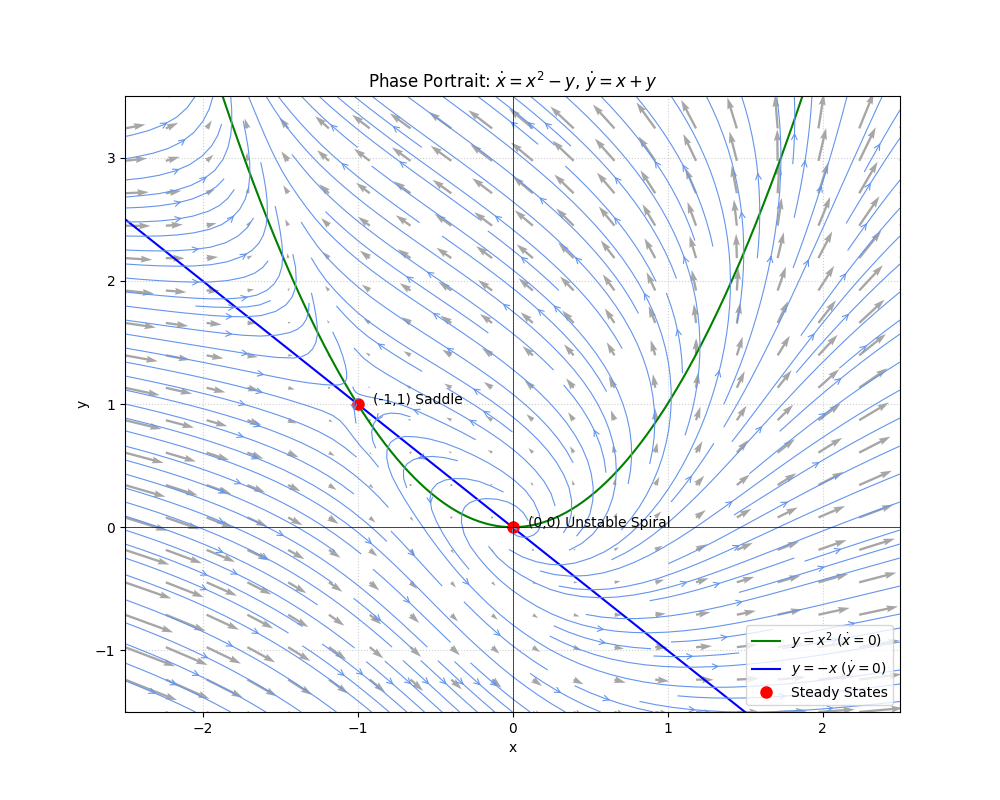
\includegraphics[width=0.8\textwidth]{phase_portrait_1.png}
\end{figure}



%%%%%%%%%%%%%%%%%%%%%%%%%%%%%%%%%%%
%%%			Task 2 ODE			%%%
%%%%%%%%%%%%%%%%%%%%%%%%%%%%%%%%%%%

\subsection*{2 Exercise}

\textit{Consider the system of nonlinear differential equations:
\begin{center}
\begin{align*}
	\frac{dx}{dt} & = \dot{x} =  x^2 - 1 & \hspace{4em} & \rlap{\footnotesize (Non-linear)} \\
	\frac{dy}{dt} & = \dot{y} =  2y      & \hspace{4em} & \rlap{\footnotesize (Linear)} \\
\end{align*}
\end{center}
}



%%%%%%%%%%%%%%%%%%%
%%%	Task 2a)	%%%
%%%%%%%%%%%%%%%%%%%

\subsubsection*{2a)}

\begin{center}
Nullcline for the first equation of the given ODE: $\dot{x} = 0$
\begin{align*}
	0   & = x^2 - 1 				&				&  \\
	x^2 & = 1 						&				&  \\
	x   & = 1 ~ \mathrm{or} ~ x=-1  & \hspace{4em} 	& \rlap{\footnotesize (Nullcline)} \\
\end{align*}
\end{center}


\begin{center}
Nullcline for the second equation of the given ODE: $\dot{y} = 0$
\begin{align*}
	0  & = 2y &					&  \\
	2y & = 0  &					&  \\
	 y & = 0  & \hspace{4em}	& \rlap{\footnotesize (Nullcline)} \\
\end{align*}
\end{center}

Steady states are states where nullclines of the system intersect, i.e. where all derivatives of the ODE system are zero.
In this case as both equations of the ODE only contain one variable we can directly conclude the steady states from the determined nullclines.
\\
The steady states of this ODE are $(1,0)$ and $(-1,0)$.



%%%%%%%%%%%%%%%%%%%
%%%	Task 2b)	%%%
%%%%%%%%%%%%%%%%%%%

\subsubsection*{2b)}

We first rewrite our ODE as a vector of functions:

\[
f(x,y) ~=~ \left[ \begin{array}{c} f_1(x,y) \\ f_2(x,y) \end{array} \right] ~=~ \left[ \begin{array}{c} x^2 - 1 \\ 2y \end{array} \right]
\]

Our functions are sufficiently differentiable, therefore we can proceed.
\\ \\
Following the definition of the Jacobi matrix, for the given ODE we thus have the following matrix:

\[
J(x,y) ~=~ \frac{\partial f}{\partial x}(a) ~=~
\begin{bmatrix}
  \frac{\partial f_1}{\partial x} & \frac{\partial f_1}{\partial y} \\[1ex] % <-- 1ex more space between rows of matrix
  \frac{\partial f_2}{\partial x} & \frac{\partial f_2}{\partial y}
\end{bmatrix}
\]

We now calculate the partial derivatives:

\begin{center}
\begin{align*}
	\frac{\partial f_1}{\partial x} &= \frac{\partial}{\partial x}(x^2 - 1) &= & 2x \\
	\frac{\partial f_1}{\partial y} &= \frac{\partial}{\partial y}(x^2 - 1) &= & 0 \\
	\frac{\partial f_2}{\partial x} &= \frac{\partial}{\partial x}(2y)	&= & 0 \\
	\frac{\partial f_2}{\partial y} &= \frac{\partial}{\partial y}(2y)	&= & 2 \\
\end{align*}
\end{center}

Having determined the partial derivatives we can write the completed Jacobi matrix:

\[
J(x,y) ~=~
\begin{bmatrix}
  2x & 0 \\[1ex] % <-- 1ex more space between rows of matrix
  0 & 2
\end{bmatrix}
\]

Finally we can evaluate the Jacobi matrix at the previously determined steady states $(1,0)$ and $(-1,0)$:

\[
J(1,0) 
~=~
\begin{bmatrix}
  2*1 & 0 \\[1ex] % <-- 1ex more space between rows of matrix
  0 & 2
\end{bmatrix}
~=~
\begin{bmatrix}
  2 & 0 \\[1ex] % <-- 1ex more space between rows of matrix
  0 & 2
\end{bmatrix}
\]

\[
J(-1,0) 
~=~
\begin{bmatrix}
  2*(-1) & 0 \\[1ex] % <-- 1ex more space between rows of matrix
  0 & 2
\end{bmatrix}
~=~
\begin{bmatrix}
  -2 & 0 \\[1ex] % <-- 1ex more space between rows of matrix
  0 & 2
\end{bmatrix}
\]


%%%%%%%%%%%%%%%%%%%
%%%	Task 2c)	%%%
%%%%%%%%%%%%%%%%%%%

\subsubsection*{2c)}

Since the Jacobian matrices are diagonal, the eigenvalues are simply the diagonal entries.
\\
\\
For the steady state $(1,0)$:
\\
The Jacobian matrix is $J(1,0) = \begin{bmatrix} 2 & 0 \\ 0 & 2 \end{bmatrix}$.
\\
The eigenvalues are $\lambda_1 = 2$ and $\lambda_2 = 2$.
\\
Since both eigenvalues are real, positive, and equal, the steady state $(1,0)$ is an \textbf{unstable star point or improper node}.
\\
\\
For the steady state $(-1,0)$:
\\
The Jacobian matrix is $J(-1,0) = \begin{bmatrix} -2 & 0 \\ 0 & 2 \end{bmatrix}$.
\\
The eigenvalues are $\lambda_1 = -2$ and $\lambda_2 = 2$.
\\
Since the eigenvalues are real and have opposite signs ($\lambda_1 < 0$, $\lambda_2 > 0$), the steady state $(-1,0)$ is a \textbf{saddle point}.


%%%%%%%%%%%%%%%%%%%
%%%	Task 2d)	%%%
%%%%%%%%%%%%%%%%%%%

\subsubsection*{2d)}

We implemented the ODE in Python and drew the phase portrait:

\begin{figure}[H]
    \centering
    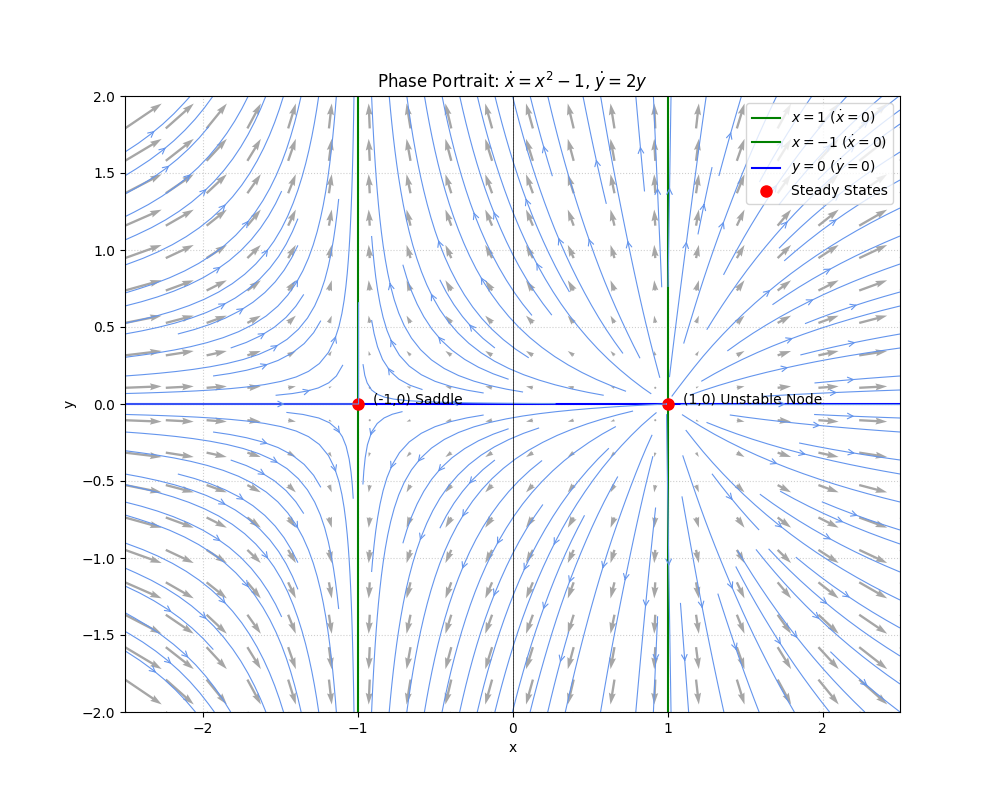
\includegraphics[width=0.8\textwidth]{phase_portrait_2.png}
\end{figure}
\end{document}



